\documentclass{article}

% Language setting
% Replace `english' with e.g. `spanish' to change the document language
\usepackage[english]{babel}

% Set page size and margins
% Replace `letterpaper' with `a4paper' for UK/EU standard size
\usepackage[letterpaper,top=2cm,bottom=2cm,left=3cm,right=3cm,marginparwidth=1.75cm]{geometry}

% Useful packages
\usepackage{amsmath}
\usepackage{amssymb}
\usepackage{amsfonts}
\usepackage{cancel}
\usepackage{graphicx}
\usepackage[colorlinks=true, allcolors=blue]{hyperref}

\usepackage{natbib}

\title{Evolutionary Pair HMM}
\author{Ian Holmes}

\begin{document}
%\maketitle

\section{Statistical alignment}

\subsection{Transducer composition}

\newcommand\gappedalphabet{(\Omega \cup \{\epsilon\})}

For our purposes, a transducer is a tuple
$\mathbb{T} = (\Omega, \Phi, \phi_0, \Psi, \tau, {\cal W})$
where
$\Omega$ is an alphabet,
$\Phi$ is a set of states,
$\phi_0 \in \Phi$ is the start state,
$\Psi \subseteq \Phi$ are the end states,
$\tau \subseteq \Phi \times \gappedalphabet \times \gappedalphabet \times \Phi$ is the transition relation, and
${\cal W}:\tau \to \Re$ is the transition weight function.

A transition $(i,x,y,j)$ has source state $i$, input label $x$, output label $y$, and destination state $j$.
For two sequences ${\cal X}, {\cal Y} \in \Omega^\ast$ define the Forward weight $\mathbb{T}_{\cal XY}$ to be the sum of weights of all paths from $\phi_0$ to any $\psi \in \Psi$
such that the concatenated input and output labels are, respectively, ${\cal X}$ and ${\cal Y}$, where the weight of a path is defined as the product of its transition weights.
Two transducers $\mathbb{A}=(\Omega,\ldots), \mathbb{B}=(\Omega,\ldots)$ are considered equivalent if $\mathbb{A}_{\cal XY} = \mathbb{B}_{\cal XY}\ \forall\ {\cal X},{\cal Y} \in \Omega^\ast$.

A transition is an ``input'' if its input label is not $\epsilon$, and ``null'' if both its input and output labels are $\epsilon$.
The ``outgoing transitions'' of a state are all the finite-weight transitions whose source is that state.
A state ``waits'' if all its outgoing transitions are inputs
and ``continues'' if (i) it's not an end state and (ii) none of its outgoing transitions are inputs.
A transducer is a ``waiting machine'' if all its states either wait or continue.
Any transducer can be transformed into an equivalent waiting machine by adding states and null transitions to split any state that doesn't meet the requirement.

A composition of two transducers $\mathbb{A},\mathbb{B}$ is a transducer $\mathbb{AB}$ representing the matrix product
\[
(\mathbb{AB})_{{\cal XZ}} = \sum_{{\cal Y} \in \Omega^\ast} \mathbb{A}_{\cal XY} \mathbb{B}_{\cal YZ} \ \forall\ {\cal X},{\cal Z} \in \Omega^\ast
\]
To establish the existence of at least one such transducer it's sufficient to consider the case where $\mathbb{B}$ is a waiting machine.
Take the Cartesian product of $\mathbb{A}$'s and $\mathbb{B}$'s state spaces and synchronize transitions,
so that $\mathbb{A}$'s output labels match $\mathbb{B}$'s input labels and $\mathbb{B}$ must be in a wait state before $\mathbb{A}$ can transition
\[
  {\cal W}_{\mathbb{AB}}((i,i'),x,z,(j,j')) = \left\{
  \begin{array}{ll}
    {\cal W}_{\mathbb{A}}(i,x,\epsilon,j) + \displaystyle \sum_{y \in \Omega} {\cal W}_{\mathbb{A}}(i,x,y,j) {\cal W}_{\mathbb{B}}(i',y,\epsilon,i') & \mbox{if $i'$ waits, $j' = i'$, and $z = \epsilon$} \\
    \displaystyle \sum_{y \in \Omega} {\cal W}_{\mathbb{A}}(i,x,y,j) {\cal W}_{\mathbb{B}}(i',y,z,j') & \mbox{if $i'$ waits and $j' \neq i'$} \\
    {\cal W}_{\mathbb{B}}(i',\epsilon,z,j') & \mbox{if $i'$ continues, $j = i$, and $x = \epsilon$} \\
    0 & \mbox{otherwise}
  \end{array} \right.
\]

\subsection{State-based emissions}

A transducer has state-based emissions if its state space can be partitioned into
match, insert, delete, and null states $\{ \sigma_M, \sigma_I, \sigma_D, \sigma_N \}$
such that for all transitions $(i,x,y,j)$ of finite weight, exactly one of the following is true
\begin{eqnarray*}
  j \in \sigma_M: & x \in \Omega, & y \in \Omega \\
  j \in \sigma_I: & x = \epsilon, & y \in \Omega \\
  j \in \sigma_D: & x \in \Omega, & y = \epsilon \\
  j \in \sigma_N: & x = \epsilon, & y = \epsilon
\end{eqnarray*}
and further ${\cal W}(i,x,y,j) = U_{ij} E_j(x,y)$ where ${\bf U}$ is a transition matrix and $E_j$ an emission weight.

Any transducer can be transformed into an equivalent state-based emitter by adding states.

\subsection{Expected transition count $T_{XY}$}

Given a probabilistically-weighted state-based emitter with exactly one match state $\sigma_M = \{ 1 \}$, which is also the start and sole end state,
we seek $T_{XY}$, the expected number of times that the shortest closed walk from/to state 1,
with its null states removed, includes a transition from $\sigma_X$ to $\sigma_Y$.

\newcommand\nottomatch{L}
\newcommand\notfrommatch{R}
\newcommand\tox{X}
\newcommand\tonull{N}
\newcommand\xtoy{{X \to Y}}

Define some indicator matrices
${\bf J}^\xtoy$,
${\bf J}^\tox$
(for $X,Y \in \{ M, I, D, N \}$) and
${\bf J}^\nottomatch$,
${\bf J}^\notfrommatch$

\begin{eqnarray*}
  J^\xtoy_{ij} & = & \left\{ \begin{array}{ll} 1 & \mbox{if $i \in \sigma_X$ and $j \in \sigma_Y$} \\ 0 & \mbox{if $i \notin \sigma_X$ or $j \notin \sigma_Y$} \end{array} \right. \\
  J^\tox_{ij} & = & \left\{ \begin{array}{ll} 1 & \mbox{if $j \in \sigma_X$} \\ 0 & \mbox{if $j \notin \sigma_X$} \end{array} \right. \\
  J^\nottomatch_{ij} & = & \left\{ \begin{array}{ll} 1 & \mbox{if $j \notin \sigma_M$} \\ 0 & \mbox{if $j \in \sigma_M$} \end{array} \right. \\
  J^\notfrommatch_{ij} & = & \left\{ \begin{array}{ll} 1 & \mbox{if $i \notin \sigma_M$} \\ 0 & \mbox{if $i \in \sigma_M$} \end{array} \right.
\end{eqnarray*}

Let ${\bf U}$ be the transition matrix.
Then

\begin{eqnarray*}
T_{XY} & = &
\left(
\left( {\bf I} - {\bf J}^\nottomatch \otimes {\bf U} \right)^{-1}
\left(
     {\bf J}^\xtoy \otimes
     \left(
     \left( {\bf I} - {\bf J}^\tonull \otimes {\bf U} \right)^{-1}
          {\bf U}
     \right)
\right)
\left( {\bf I} - {\bf J}^\notfrommatch \otimes {\bf U} \right)^{-1}
\right)_{11}
\end{eqnarray*}

Here $\otimes$ is the elementwise product.



\subsection{Rate of change $R_{XY}$ of expected transition count}

Suppose that
$\mathbb{Q}(\theta)$ is the generator for an indel process,
$\mathbb{G}(\theta,\delta_t) = \mathbb{I} + \mathbb{Q}(\theta) \delta_t$ is the infinitesimal Pair HMM,
$\mathbb{F}(t)$ the finite-time approximator,
and $\mathbb{FG}$ the composition of $\mathbb{F}$ and $\mathbb{G}$.

Let ${\bf U}(\theta,t,\delta_t)$ be the transition matrix
of the composite machine $\mathbb{FG}$
at time $t$, infinitesimal time increment $\delta_t$, and parameter value $\theta$.
By the definition of $\mathbb{G}$ this is first-order in $\delta_t$, so it has the form
\[
  {\bf U}(\theta,t,\delta_t) = {\bf U}_0(\theta,t) + {\bf U}_t(\theta,t) \delta_t
  \]

We are interested in
\begin{eqnarray*}
\frac{\partial}{\partial t}T_{XY} & = & \lim_{\delta_t \to 0} \frac{T_{XY}(\theta,t,\delta_t) - T_{XY}(\theta,t,0)}{\delta_t} \\
\frac{\partial^2}{\partial \theta \partial t}T_{XY} & = & \lim_{\delta_\theta \to 0} \lim_{\delta_t \to 0}
\frac{\left(T_{XY}(\theta+\delta_\theta,t,\delta_t) - T_{XY}(\theta+\delta_\theta,t,0)\right) - \left(T_{XY}(\theta,t,\delta_t) - T_{XY}(\theta,t,0)\right)}{\delta_\theta \delta_t}
\end{eqnarray*}
We will use the time derivative to numerically integrate $T_{XY}$, and the cross partial derivative for parameter-fitting.
For later convenience define $R_{XY} \equiv \frac{\partial}{\partial t} T_{XY}$.

Expand ${\bf U}$ to first order in both $\delta_\theta$ and $\delta_t$
\newcommand\tthetaexpansion[2]{  {#2}_0^{#1}
  + {#2}_\theta^{#1} \delta_\theta
  + {#2}_t^{#1} \delta_t
  + {#2}_{\theta t}^{#1} \delta_\theta \delta_t }
\newcommand\uexpansion{\tthetaexpansion{}{\bf U}}
\newcommand\vexpansion[1]{\tthetaexpansion{#1}{\bf V}}
\[
  {\bf U}(\theta+\delta_\theta,t,\delta_t) = \uexpansion + O(\delta_\theta^2) % + O(\delta_t^2)
\]
where ${\bf U}_0={\bf U}(\theta,t,0)$,
${\bf U}_t=\frac{1}{\delta_t} \left( {\bf U}(\theta,t,\delta_t) - {\bf U}(\theta,t,0) \right)$,
${\bf U}_\theta=\frac{\partial}{\partial \theta} {\bf U}_0$,
${\bf U}_{\theta t}=\frac{\partial}{\partial \theta}  {\bf U}_t$.

We can now expand the matrix inverses.
In general, for $x \in \{ \nottomatch, \tonull, \notfrommatch \}$,
\begin{eqnarray*}
  \left( {\bf I} - {\bf J}^x \otimes {\bf U} \right)^{-1}
%  & = &
%  \left( {\bf I} - {\bf J}^x \otimes {\bf U}_0
%  - {\bf J}^x \otimes {\bf U}_\theta \delta_\theta
%  - {\bf J}^x \otimes {\bf U}_t \delta_t
%  - {\bf J}^x \otimes {\bf U}_{\theta t} \delta_\theta \delta_t
%  + O(\delta_\theta^2) + O(\delta_t^2)
%  \right)^{-1} \\
%  & = &
%  \left(
%  \left( {\bf I} - {\bf J}^x \otimes {\bf U}_0 \right)
%  \left( {\bf I}
%  - {\bf V}^x_0 \left( {\bf J}^x \otimes {\bf U}_\theta \delta_\theta
%  + {\bf J}^x \otimes {\bf U}_t \delta_t
%  + {\bf J}^x \otimes {\bf U}_{\theta t} \delta_\theta \delta_t
%  \right) \right)
%  + O(\delta_\theta^2) + O(\delta_t^2)
%  \right)^{-1} \\
%  & = &
%  \left(
%  \left( {\bf I}
%  + {\bf V}^x_0 \left( {\bf J}^x \otimes {\bf U}_\theta \delta_\theta
%  + {\bf J}^x \otimes {\bf U}_t \delta_t
%  + {\bf J}^x \otimes {\bf U}_{\theta t} \delta_\theta \delta_t
%  \right)
%  \right) \right)
%  {\bf V}^x_0
%  + O(\delta_\theta^2) + O(\delta_t^2) \\
%  & = &
%  {\bf V}^x_0
%  + {\bf V}^x_0 \left( {\bf J}^x \otimes {\bf U}_\theta \right) {\bf V}^x_0 \delta_\theta
%  + {\bf V}^x_0 \left( {\bf J}^x \otimes {\bf U}_t \right) {\bf V}^x_0 \delta_t
%  + {\bf V}^x_0 \left( {\bf J}^x \otimes {\bf U}_{\theta t} \right) {\bf V}^x_0 \delta_\theta \delta_t
%  + O(\delta_\theta^2) + O(\delta_t^2) \\
  & = & \vexpansion{x} + O(\delta_\theta^2) + O(\delta_t^2) \\
{\bf V}^x_0 & = & ({\bf I} - {\bf J} \otimes {\bf U}_0)^{-1} \\
{\bf V}^x_\theta & = & {\bf V}^x_0 \left( {\bf J} \otimes {\bf U}_\theta \right) {\bf V}^x_0 \\
{\bf V}^x_t & = & {\bf V}^x_0 \left( {\bf J} \otimes {\bf U}_t \right) {\bf V}^x_0 \\
{\bf V}^x_{\theta t} & = & {\bf V}^x_0 \left( {\bf J} \otimes {\bf U}_{\theta t} \right) {\bf V}^x_0
\end{eqnarray*}

Thus
\begin{eqnarray*}
T_{XY} & = &
\left(
\left( \vexpansion\nottomatch \right)
\right. \\ & & \quad \times
\left(
     {\bf J}^\xtoy \otimes
     \left( \left( \vexpansion\tonull \right)
     \left( \uexpansion \right) \right)
\right)
 \\ & & \quad \left. \times
 \left( \vexpansion\notfrommatch \right)
\right)_{11}  + O(\delta_\theta^2) + O(\delta_t^2)
\end{eqnarray*}

For convenience define
\begin{eqnarray*}
W_{a,b,c,d} & = &
\left( {\bf V}^\nottomatch_a \left( {\bf J}^\xtoy \otimes \left( {\bf V}^\tonull_b {\bf U}_c \right) \right) {\bf V}^\notfrommatch_d \right)_{11}
\end{eqnarray*}
Examining the coefficients of $\delta_t$ and $\delta_\theta \delta_t$, we see that

\begin{eqnarray*}
  R_{XY} & = &
  W_{t,0,0,0} + W_{0,t,0,0} + W_{0,0,t,0} + W_{0,0,0,t}
  \\
  \frac{\partial}{\partial \theta}R_{XY} & = &
  W_{t,\theta,0,0} + W_{t,0,\theta,0} + W_{t,0,0,\theta}
  + W_{\theta,t,0,0} + W_{0,t,\theta,0} + W_{0,t,0,\theta}
  + W_{\theta,0,t,0} + W_{0,\theta,t,0} + W_{0,0,t,\theta}
  \\ & &
  + W_{\theta,0,0,t} + W_{0,\theta,0,t} + W_{0,0,\theta,t}
  + W_{\theta t,0,0,0} + W_{0,\theta t,0,0} + W_{0,0,\theta t,0} + W_{0,0,0,\theta t}
\end{eqnarray*}

This first-order expansion allows us to ``differentiate through'' the matrix inverse.
These equations remain valid if the parameter $\theta$, with respect to which we are differentiating, is itself one of the $T_{XY}$
(since these are parameters of $\mathbb{F}(t)$ and hence of ${\bf U}$).

\subsection{Expected state count $S_X$}

We will also need $S_X$, the expected number of $\sigma_X$-states in the walk.
Note that $S_x = \sum_{y \in \{M,I,D\}} T_{xy}  = \sum_{y \in \{M,I,D\}} T_{yx}$
and $S_M = 1$.
Thus if we have all the $\{ T_{XY} \}$ then we can trivially find the $\{ S_X \}$.
However, sometimes it will be useful to compute the $S_X$ independently,
as for example in the GGI model below, where it is easier to solve ODEs for the $S_X$ than the $T_{XY}$.

\begin{eqnarray*}
S_X & = &
\left(
     \left(
          {\bf J}^\tox \otimes
          \left( {\bf I} - {\bf J}^\nottomatch \otimes {\bf U} \right)^{-1}
     \right)
\left( {\bf I} - {\bf J}^\notfrommatch \otimes {\bf U} \right)^{-1}
\right)_{11}
\\
& = &
\left(
     \left(
          {\bf J}^\tox \otimes
          \left( \vexpansion\nottomatch \right)
     \right)
\left( \vexpansion\notfrommatch \right)
\right)_{11}  + O(\delta_\theta^2) + O(\delta_t^2)
  \\
  \frac{\partial}{\partial t} S_X & = &
  W'_{t,0} + W'_{0,t}
  \\
  \frac{\partial^2}{\partial \theta \partial t} S_X & = &
  W'_{t,\theta} + W'_{\theta,t}
  + W'_{\theta t,0} + W'_{0,\theta t}
\\
W'_{a,b} & = &
\left( \left( {\bf J}^\tox \otimes {\bf V}^\nottomatch_a \right) {\bf V}^\notfrommatch_b \right)_{11}
\end{eqnarray*}


\subsection{Runge-Kutta recursions for $T_{XY}$ and derivatives}

Let $\Theta$ denote the parameters of $\mathbb{G}(\delta_t)$
while ${\bf T}(t)$, including all the $T_{XY}(t)$, parameterizes $\mathbb{F}(t)$.

We want to use the Runge-Kutta method (RK4) to numerically estimate $T_{XY}$ at timepoints $(t_0=0, t_1, t_2 \ldots)$.
Let $\Delta_n = t_{n+1}-t_n$.
Applying the RK4 method gives

\begin{eqnarray*}
  {\bf T}^{(n+1)} & = & {\bf T}^{(n)} + \frac{\Delta_n}{6} \left( {\bf K}^{(n,1)} + 2{\bf K}^{(n,2)} + 2{\bf K}^{(n,3)} + {\bf K}^{(n,4)} \right) \\
  {\bf K}^{(n,1)} & = & {\bf R}\left(\Theta,{\bf T}^{(n)}\right) \\
  {\bf K}^{(n,2)} & = & {\bf R}\left(\Theta,{\bf T}^{(n)} + \frac{\Delta_n}{2} {\bf K}^{(n,1)}\right) \\
  {\bf K}^{(n,3)} & = & {\bf R}\left(\Theta,{\bf T}^{(n)} + \frac{\Delta_n}{2} {\bf K}^{(n,2)}\right) \\
  {\bf K}^{(n,4)} & = & {\bf R}\left(\Theta,{\bf T}^{(n)} + \Delta_n {\bf K}^{(n,3)}\right)
\end{eqnarray*}

For any parameter $\theta \in \Theta$ we can use the chain rule to find the derivative

\newcommand\ptheta{\frac{\partial}{\partial\theta}}
\newcommand\ptxy{\frac{\partial}{\partial T_{XY}}}
\newcommand\allpartials[1]{\ptheta #1 + \sum_{X,Y} \ptxy #1 \ptheta T_{XY}^{(n)}}
\newcommand\allpartialsk[3]{\ptheta #1 + \sum_{X,Y} \ptxy #1 \left( \ptheta T_{XY}^{(n)} + #2 \ptheta K_{XY}^{(n,#3)} \right)}
\begin{eqnarray*}
  \ptheta {\bf T}^{(n+1)} & = & \ptheta {\bf T}^{(n)} + \frac{\Delta_n}{6} \left( \ptheta {\bf K}^{(n,1)} + 2\ptheta{\bf K}^{(n,2)} + 2\ptheta{\bf K}^{(n,3)} + \ptheta{\bf K}^{(n,4)} \right) \\
  \ptheta {\bf K}^{(n,1)} & = & \allpartials{{\bf R}\left(\Theta,{\bf T}^{(n)}\right)} \\
  \ptheta {\bf K}^{(n,2)} & = & \allpartialsk{{\bf R}\left(\Theta,{\bf T}^{(n)} + \frac{\Delta_n}{2} {\bf K}^{(n,1)}\right)}{\frac{\Delta_n}{2}}{1} \\
  \ptheta {\bf K}^{(n,3)} & = & \allpartialsk{{\bf R}\left(\Theta,{\bf T}^{(n)} + \frac{\Delta_n}{2} {\bf K}^{(n,2)}\right)}{\frac{\Delta_n}{2}}{2} \\
  \ptheta {\bf K}^{(n,4)} & = & \allpartialsk{{\bf R}\left(\Theta,{\bf T}^{(n)} + \Delta_n {\bf K}^{(n,3)}\right)}{\Delta_n}{3}
\end{eqnarray*}

\subsection{Generator $\mathbb{G}(\delta_t)$ for General Geometric Indel model (GGI)}

A sequence ${\cal S}(t)$ evolves by
substitutions (rate matrix ${\bf Q}$),
deletions (rate $\mu$ per site, extension probability $y$),
and
insertions (rate $\lambda$, extension $x$,
characters $\sim {\bf Q}$'s stationary distribution $\pi$).

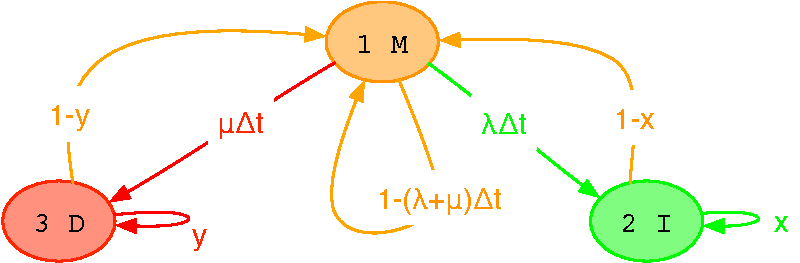
\includegraphics[width=\textwidth]{InstantHMM.pdf}

At equilibrium, sequence length $\sim$ Geometric($\lambda/\mu$). Character frequencies $\pi$.

If the model is required to be reversible then $\lambda y(1-x) = \mu x(1-y)$.

\subsection{Approximate time-dependent transducer $\mathbb{F}(t)$ for GGI model}

A Pair HMM whose Forward likelihood approximates $P({\cal S}(t)|{\cal S}(0))$

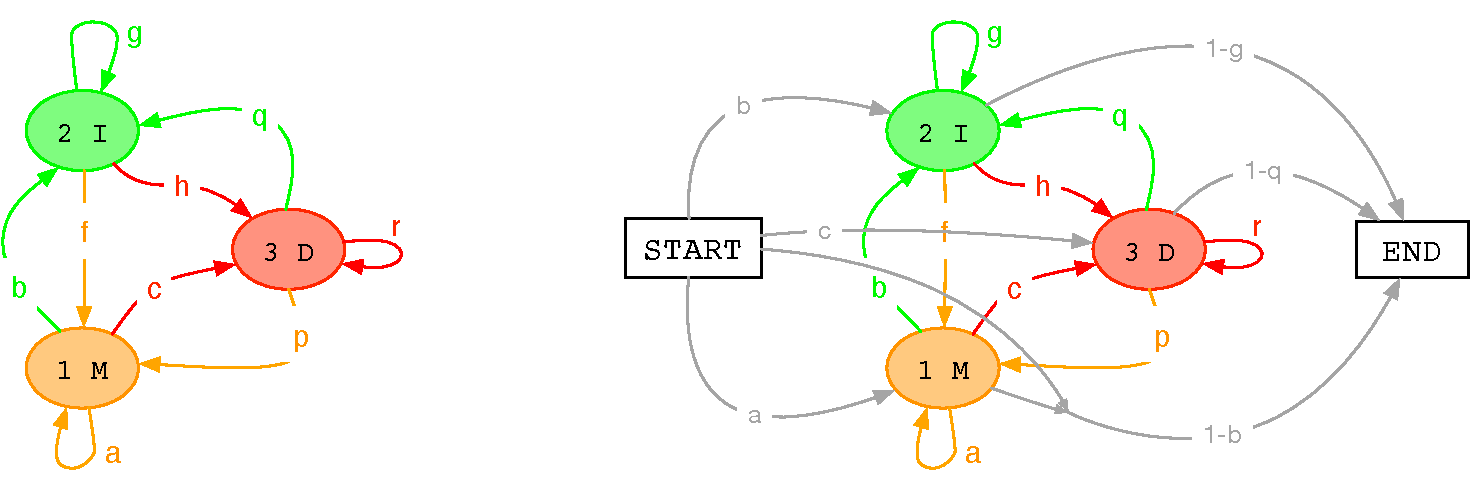
\includegraphics[width=\textwidth]{PairHMM.pdf}

At $t=0$: $a(0)=1$, $f(0)=1-x$, $g(0)=x$, $p(0)=1-y$, $r(0)=y$, and $b(0)=c(0)=h(0)=q(0)=0$.

For $t>0$, % following Holmes (2020)
\begin{eqnarray*}
\begin{pmatrix}
a & b & c \\
f & g & h \\
p & q & r 
\end{pmatrix}
& = &
\begin{pmatrix}
T_{MM} / S_M & T_{MI} / S_M & T_{MD} / S_M \\
T_{IM} / S_I & T_{II} / S_I & T_{ID} / S_I \\
T_{DM} / S_D & T_{DI} / S_D & T_{DD} / S_D 
\end{pmatrix}
\\
& = &
\begin{pmatrix}
T_{MM} & T_{MI} & 1-T_{MM}-T_{MI} \\
T_{IM}/S_I & (S_I-T_{MI}-T_{DI})/S_I & (T_{MI}+T_{DI}-T_{IM})/S_I \\
(1-T_{MM}-T_{IM})/S_D & T_{DI}/S_D & (S_D+T_{MM}+T_{IM}-T_{DI}-1)/S_D 
\end{pmatrix}
\end{eqnarray*}

\subsection{Composite machine $\mathbb{FG}$ for GGI model}

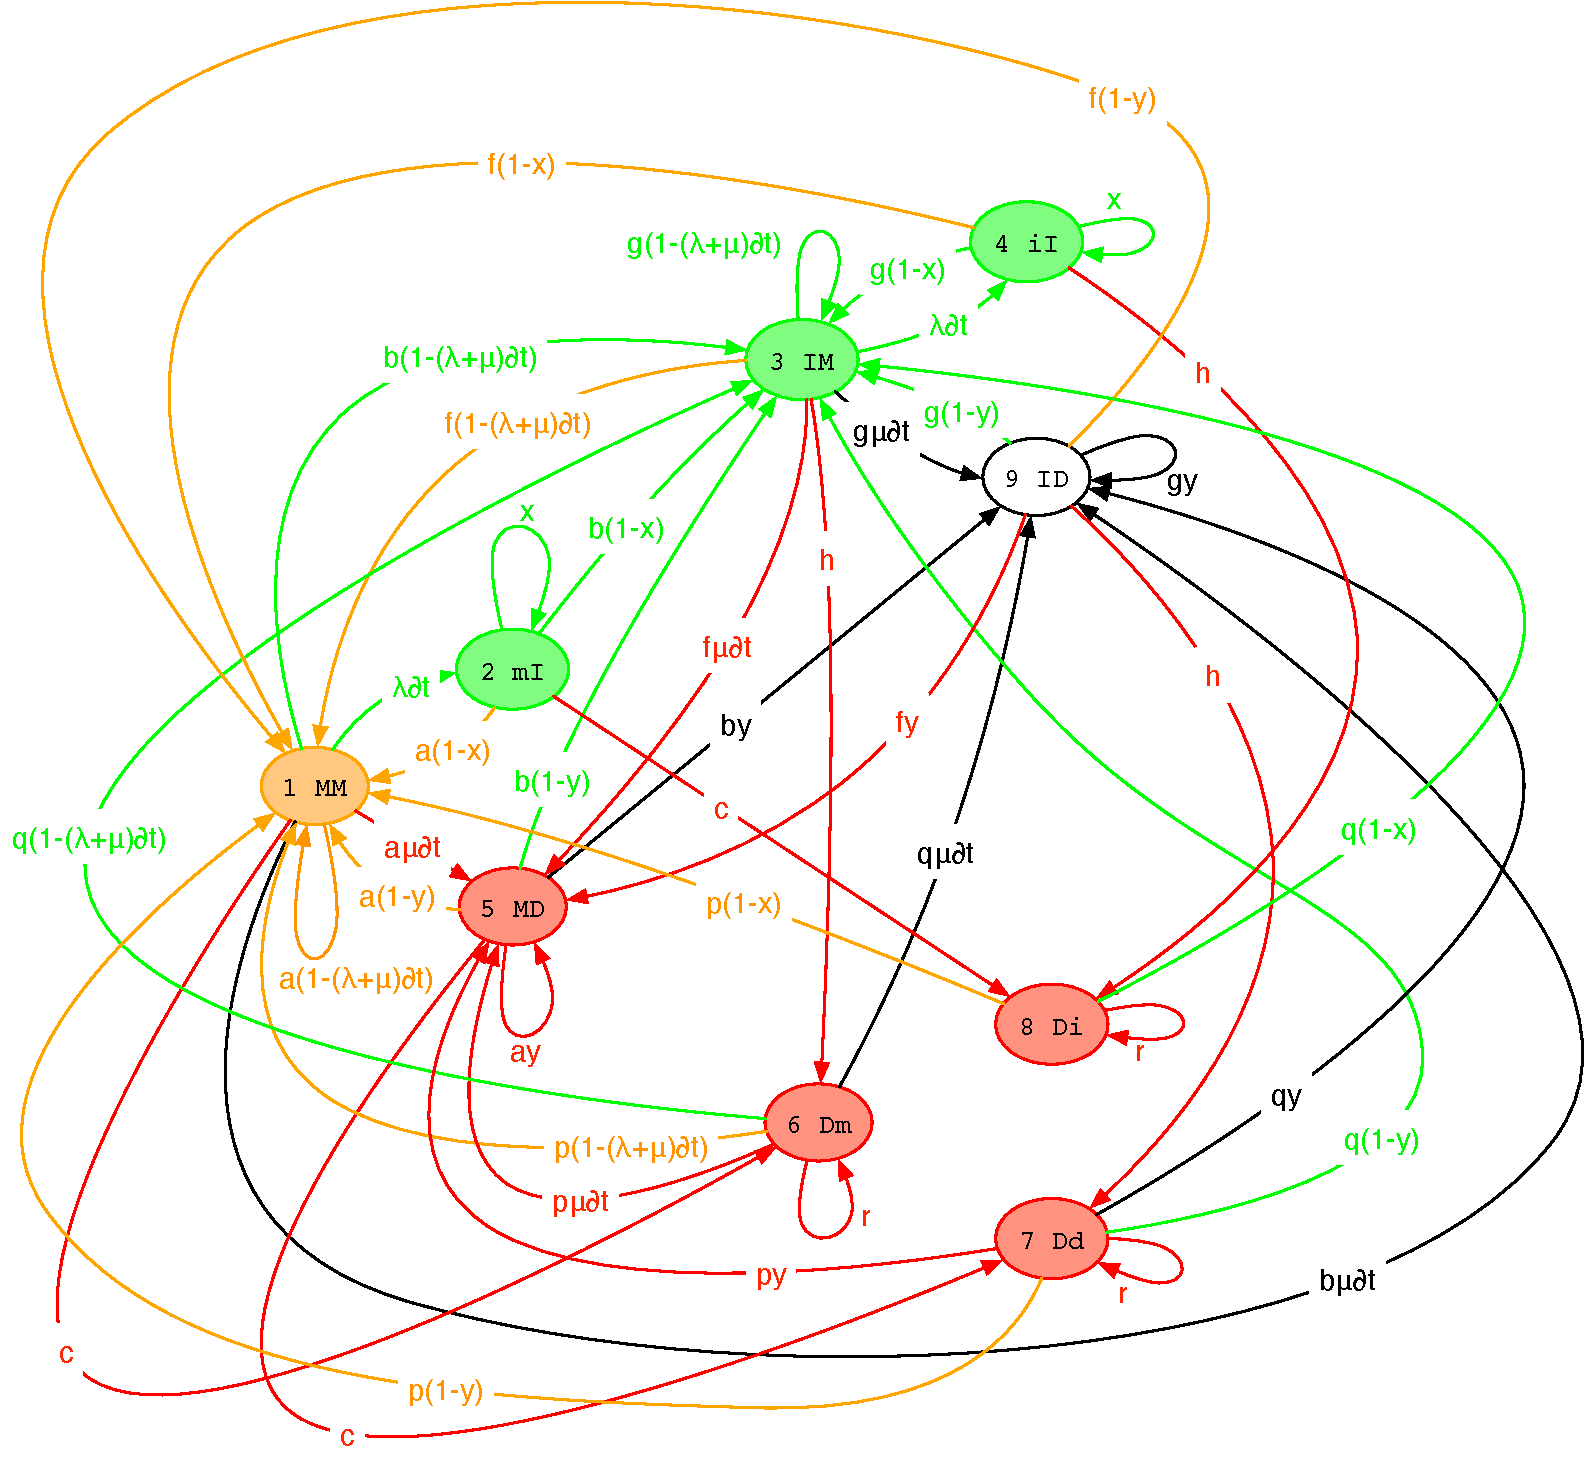
\includegraphics[width=\textwidth]{PairInstant.pdf}

\[
 {\bf U} =
  \begin{pmatrix}
a (1-(\lambda+\mu) \delta_t) & \lambda \delta_t & b (1-(\lambda+\mu) \delta_t) & 0 & a \mu \delta_t & c & 0 & 0 & b \mu \delta_t \\
a (1-x) & x & b (1-x) & 0 & 0 & 0 & 0 & c & 0 \\
f (1-(\lambda+\mu) \delta_t) & 0 & g (1-(\lambda+\mu) \delta_t) & \lambda \delta_t & f \mu \delta_t & h & 0 & 0 & g \mu \delta_t \\
f (1-x) & 0 & g (1-x) & x & 0 & 0 & 0 & h & 0 \\
a (1-y) & 0 & b (1-y) & 0 & a y & 0 & c & 0 & b y \\
p (1-(\lambda+\mu) \delta_t) & 0 & q (1-(\lambda+\mu) \delta_t) & 0 & p \mu \delta_t & r & 0 & 0 & q \mu \delta_t \\
p (1-y) & 0 & q (1-y) & 0 & p y & 0 & r & 0 & q y \\
p (1-x) & 0 & q (1-x) & 0 & 0 & 0 & 0 & r & 0 \\
f (1-y) & 0 & g (1-y) & 0 & f y & 0 & h & 0 & g y    
  \end{pmatrix}
\]

State sets are
$\sigma_M=\{1\}$ (orange),
$\sigma_I=\{2,3,4\}$ (green),
$\sigma_D=\{5,6,7,8\}$ (red),
$\sigma_N=\{9\}$ (white).
  
\subsection{Algebraic ODEs for $T_{XY}$ under GGI model}

Derived in \cite{Holmes2020}.

\begin{eqnarray*}
S_I(t) & = & \exp\left(\frac{\lambda t}{1-x}\right)-1 \\
S_D(t) & = & \exp\left(\frac{\mu t}{1-y}\right)-1 \\
T_{ij}(0) & = & \mbox{1 if $i=j=M$, 0 otherwise}
\\
  \frac{d}{dt} T_{MM}(t) & = &
  \mu \frac{b f (1-y)}{1 - g y}-(\lambda +\mu )a
  \nonumber \\
  \frac{d}{dt} T_{MI}(t) & = &
  -\mu \frac{b (1-g)}{1 - g y} + \lambda (1-b)
  \nonumber \\
  \frac{d}{dt} T_{IM}(t) & = &
  \lambda a - \mu \frac{f (1-g) (b (1-r)+c q)}{(1 - g y) (f (1-r)+h p)}
  \nonumber \\
  \frac{d}{dt} T_{DI}(t) & = &
  \mu \frac{(1-g) (b (1-r-h q)+c g q)}{(1-g y) (f (1-r)+h p)}
\end{eqnarray*}

The substitution matrix $E_M(x,y)$ for the match state is
the matrix exponential $\exp({\bf Q}t)_{xy}$, for which a Pad\'{e} approximant
or other power series expansion can be used in order to remain automatically differentiable under frameworks like PyTorch or Jax. % \cite{MolerVanLoan2003}
For the insert states the emission weights are $E_I(\epsilon,y)=\pi_y$,
and for the delete states $E_D(x,\epsilon)=1$.

\subsection{TKF91 as exactly-solved special case of GGI model}

When $x=y=0$ the model is TKF91 \cite{ThorneEtAl91}
with solution
$
\begin{pmatrix}
a & b & c \\
f & g & h \\
p & q & r 
\end{pmatrix}
=
\begin{pmatrix}
(1-\beta)\alpha & \beta & (1-\beta)(1-\alpha) \\
(1-\beta)\alpha & \beta & (1-\beta)(1-\alpha) \\
(1-\gamma)\alpha & \gamma & (1-\gamma)(1-\alpha)
\end{pmatrix}
$
where
$\alpha = \exp(-\mu t)$,
$\beta = \frac{\lambda \left( \exp(-\lambda t) - \exp(-\mu t) \right)}{\mu \exp(-\lambda t) - \lambda \exp(-\mu t)}$
and
$\gamma = 1 - \frac{\mu \beta}{\lambda (1 - \alpha)}$.



\subsection{GGI model transition likelihood, alignment unspecified}

Suppose a prefix list (or tree) of sequences.
Node 1 corresponds to the empty sequence.
Nodes $N>1$ correspond to nonempty sequences ${\cal S}_N$.
Character $\omega_N$ is the last character of ${\cal S}_N$.
The parent node $\psi_N$ corresponds to the longest prefix of ${\cal S}_N$:
removing $\omega_N$ from ${\cal S}_N$ leaves ${\cal S}_{\psi_N}$.

Let $F(i,j,t) = \begin{pmatrix} F_M & F_I & F_D \end{pmatrix}$
be the per-state Forward likelihoods for sequences ${\cal S}_i,{\cal S}_j$.

We seek $F^\dagger(i,j,t) = P({\cal S}(t)={\cal S}_j|{\cal S}(0)={\cal S}_i)$.
The Forward recursions are, for $i>1$ and $j>1$
\begin{eqnarray*}
F(1,1,t) & = & \begin{pmatrix} 1 & 0 & 0 \end{pmatrix}
\\
F(1,j,t) & = &
F(1,\psi_j,t) U_I(\omega_j,t)
\\
F(i,1,t) & = &
F(\psi_i,1,t) U_D(\omega_i,t)
\\
F(i,j,t) & = &
F(\psi_i,\psi_j,t) U_M(\omega_i,\omega_j,t)
+ F(i,\psi_j,t) U_I(\omega_j,t)
+ F(\psi_i,j,t) U_D(\omega_i,t)
\\
F^\dagger(i,j,t) & = & F(i,j,t) \begin{pmatrix}
1-b(t) \\
1-g(t) \\
1-q(t) \end{pmatrix}
\\
U_M(\omega_i,\omega_j,t) & = &
\begin{pmatrix}
a(t) & 0 & 0 \\
f(t) & 0 & 0 \\
p(t) & 0 & 0 
\end{pmatrix}
\exp({\bf Q}t)_{\omega_i \omega_j}
\\
U_I(\omega_j,t) & = &
\begin{pmatrix}
0 & b(t) & 0 \\
0 & g(t) & 0 \\
0 & q(t) & 0 
\end{pmatrix}
\pi_{\omega_j}
\\
U_D(\omega_i,t) & = &
\begin{pmatrix}
0 & 0 & c(t) \\
0 & 0 & h(t) \\
0 & 0 & r(t) 
\end{pmatrix}
\end{eqnarray*}

The time complexity to compute the Forward likelihood is $O(L^2)$,
where $L$ is the sequence length.

\subsection{GGI model transition likelihood, alignment specified}

The pairwise alignment of ancestor $i$ and descendant $j$ can be summarized by two lists:
\begin{itemize}
    \item The list $A_M$ of pairs of aligned characters $(\omega,\omega')$ from ancestor ${\cal S}(0)$ and descendant ${\cal S}(t)$;
    \item The list $A_{ID}$ of pairs of unaligned gap sequences $(\delta,\delta')$ that were deleted and inserted in between.
\end{itemize}

The alignment probability, computable in time $O(L)$ (and in practice very fast), is
\[
P(A_M,A_{ID},{\cal S}(t)|{\cal S}(0)) =
\prod_{(\omega,\omega') \in A_M} \exp({\bf Q}t)_{\omega \omega'}
\prod_{(\delta,\delta') \in A_{ID}} G(|\delta|,|\delta'|,t)
\prod_{\omega'\in \delta'} \pi_{\omega'}
\]

where $G(i,j,t)$ is the probability that between the next pair of aligned characters in ${\cal S}(0)$ and ${\cal S}(t)$,
there were $i$ characters deleted from ${\cal S}(0)$ 
and $j$ characters inserted into ${\cal S}(t)$,
with no homology
\begin{eqnarray*}
G(0,0,t) & = & a \\
G(i,0,t) & = & cr^{i-1}p \\
G(0,j,t) & = & bg^{j-1}f \\
G(i,j,t) & = &
g^{j-1} r^{i-1}
\sum_{k=0}^{\min(i,j)}
\left(\frac{hq}{gr}\right)^k
\left[
\binom{i}{k} \binom{j-1}{k} brf
+ \binom{i-1}{k} \binom{j-1}{k} (bhp+cqf)
+ \binom{i-1}{k} \binom{j}{k} cgp
\right]
\end{eqnarray*}
% The unobserved index $k$ counts zig-zags on the Pair HMM state path
% ($D \to I \to D$ or $I \to D \to I$).

\subsection{Phylogenetic alignment under GGI model}

Both forms of the pairwise likelihood (alignment specified, or unspecified) can be extended to multiple sequences on a phylogeny.
Upgrade $\exp({\bf Q}t)$ to Felsenstein pruning. % \cite{Felsenstein81}.

For the alignment-unspecified form, use transducer composition to obtain $N$-sequence HMMs \cite{SilvestreRyanEtAl2020}.
The resulting Forward algorithm is $O(L^N)$.
To ameliorate this, discard all but a few representative sample paths \cite{WestessonEtAl2012},
or use MCMC \cite{RedelingsSuchard2007}.

\bibliographystyle{unsrt}
\bibliography{references}


\end{document}
